\documentclass[journal]{IEEEtran}
\IEEEoverridecommandlockouts

\usepackage{cite}
\usepackage{amsmath,amssymb,amsfonts}
\usepackage{graphicx}
\usepackage{booktabs}
\usepackage{tabularx}
\usepackage{array}
\usepackage{textcomp}
\usepackage{xcolor}
\usepackage[colorlinks=true,urlcolor=blue,linkcolor=black,citecolor=black]{hyperref}

\graphicspath{{./}{Research_paper/}{./Research_paper/}}

\def\BibTeX{{\rm B\kern-.05em{\sc i\kern-.025em b}\kern-.08em
T\kern-.1667em\lower.7ex\hbox{E}\kern-.125emX}}

\begin{document}

\title{Vulnerability Scanning Using AI Based IDE Extension And Server Agent}

\author{%
\makebox[\linewidth]{%
\begin{minipage}[t]{0.30\linewidth}\centering
\textbf{Vedika Khochare}\\
\small\textit{Department of AI \& Data Science}\\
\small K.J. Somaiya Institute of Technology\\
\small Mumbai, India\\
\scriptsize\texttt{vedika.khochare@somaiya.edu}
\end{minipage}\hfill
\begin{minipage}[t]{0.30\linewidth}\centering
\textbf{Shrinidhi Malli}\\
\small\textit{Department of AI \& Data Science}\\
\small K.J. Somaiya Institute of Technology\\
\small Mumbai, India\\
\scriptsize\texttt{shrinidhi.malli@somaiya.edu}
\end{minipage}\hfill
\begin{minipage}[t]{0.30\linewidth}\centering
\textbf{Vatshal Mehta}\\
\small\textit{Department of AI \& Data Science}\\
\small K.J. Somaiya Institute of Technology\\
\small Mumbai, India\\
\scriptsize\texttt{vatshal.m@somaiya.edu}
\end{minipage}
}\\[5pt]
\makebox[\linewidth]{%
\begin{minipage}[t]{0.55\linewidth}\centering
\small\textit{Guide:} \textbf{Prof. Vidya Sagvekar}\\
\small Department of AI \& Data Science\\
\small K.J. Somaiya Institute of Technology, Mumbai\\
\scriptsize\texttt{vsagvekar@somaiya.edu}
\end{minipage}
}
}

\maketitle

\begin{abstract}

Application security is commonly divided between development-time source
analysis and post-deployment monitoring. This separation can create a
visibility gap because source-level tools may miss weaknesses that emerge
only during execution, while runtime findings may not retain sufficient
project context to explain their origin.

This paper presents \textit{SentinelAI}, a developer-centric application
security framework integrating IDE-based static analysis, optional Large
Language Model (LLM) reasoning, independent runtime attack-surface discovery,
bounded Docker-based runtime testing, evidence-based verdicts, remediation
and re-test, and a planned Server Sentinel component for post-deployment
monitoring.

The currently evaluated contribution is SentinelAI's bounded runtime-security
workflow consisting of independent runtime discovery, applicability-aware
probe planning, controlled execution, evidence normalization, and explicit
runtime verdicts. Safe Simulation evaluates this pipeline under controlled
synthetic conditions, while Project Runtime Validation applies the same
catalogue to an authorized real application.

In the measured Safe Simulation run, 35 runtime-security families produced
44 controlled probe executions. Forty-two probes produced detected outcomes
and two produced observed-exposure outcomes, resulting in 44 of 44 expected
classifications with no inconclusive or failed executions.

Project Runtime Validation was evaluated across authorized project-runtime
reports using applicability-aware testing. The reported runtime results show
that only security families supported by the discovered routes, inputs,
protocols, and application context were executed, while unsupported families
were retained as not applicable rather than being treated as failed
detections.

A 50-case report-based evaluation was additionally organized so that
individual cases could contain zero, one, or multiple known vulnerabilities.
Eighteen cases contained no known vulnerabilities and 32 contained one or
more vulnerabilities, representing 58 known vulnerability instances. Across
the reports, SentinelAI detected 55 of the 58 known vulnerability instances,
with five false-positive findings and three missed vulnerabilities. The
result corresponds to 91.67\% precision, 94.83\% recall, and 93.22\%
F1-score. At the test-case level, 17 of 18 clean cases were correctly
identified as clean, and 48 of the 50 cases were classified correctly.

\end{abstract}

\begin{IEEEkeywords}
Application Security, Static Analysis, Runtime Security, Dynamic Testing,
Large Language Models, IDE Extension, Docker, Vulnerability Validation,
Security Drift, DevSecOps
\end{IEEEkeywords}

\section{Introduction}

Modern software delivery frequently separates security analysis across
source code, runtime testing, deployment, and production monitoring.
Static Application Security Testing (SAST) can identify weaknesses before
execution, but its effectiveness is limited when vulnerability behavior
depends on runtime configuration, authentication state, deployment
conditions, or cross-component interactions~\cite{b5}.

LLMs can provide contextual security reasoning, yet independent studies show
that general-purpose models remain unreliable as standalone vulnerability
detectors~\cite{b13,b14}. Prompt injection further demonstrates why
model-generated conclusions should be treated as hypotheses rather than
security proof~\cite{b4}.

SentinelAI addresses this gap through a developer-oriented workflow that
starts inside the IDE but does not stop at source analysis. Runtime discovery
executes independently of static or AI findings, allowing runtime-only
weaknesses to be observed even when source analysis reports no findings.

SentinelAI distinguishes two runtime-testing purposes.
\textit{Safe Simulation} validates the runtime engine against controlled
synthetic conditions. \textit{Project Runtime Validation} evaluates a real
authorized application and executes only security families that are
meaningful for the discovered runtime context.

The currently evaluated contribution of SentinelAI is the bounded
runtime-security workflow consisting of independent runtime discovery,
applicability-aware planning, controlled execution, evidence normalization,
and explicit verdict classification.

The planned Server Sentinel and Control Plane extend this architecture toward
post-deployment monitoring but are not included in the current measured
implementation claims.

\section{Related Work}

\subsection{Static and AI-Assisted Vulnerability Detection}

Static analysis remains important because it can inspect software before
execution. Yuan \textit{et al.} studied static SQL-injection detection using
program transformation and taint analysis~\cite{b5}.

Generative models have also been investigated for software vulnerability
analysis~\cite{b10,b11}. Ullah \textit{et al.} show that LLMs do not yet
reliably identify and reason about vulnerabilities without additional
grounding~\cite{b13}. SentinelAI therefore keeps AI optional and does not
make runtime validation dependent on LLM output.

\subsection{Runtime Security Validation}

PentestGPT and related work demonstrate the potential of structured
LLM-assisted penetration-testing workflows~\cite{b7,b8}. OWASP ZAP provides
a mature automated dynamic-testing framework~\cite{zap}, while Nuclei
provides template-based scanning across web and network targets~\cite{nuclei}.

SentinelAI differs in its emphasis on carrying runtime evidence back into the
same project-security record used during development.

\subsection{Deployment Monitoring}

Falco, osquery, Wazuh, and Datadog provide runtime, endpoint, host, and
application monitoring capabilities~\cite{falco,osquery,wazuhagent,datadogagent}.
SentinelAI's planned Server Sentinel has a narrower objective: associating
application-facing deployment changes with the same project context used
during source and runtime analysis.

\section{Problem Statement}

Security workflows often separate static analysis, runtime validation, and
deployment monitoring. This creates several practical gaps.

Static analysis can miss weaknesses whose exploitability depends on runtime
behavior or configuration. AI reasoning can improve context but cannot be
treated as independent vulnerability proof. Runtime testing that depends
only on existing source findings can also miss runtime-only exposures.

Blindly executing every possible security payload against every endpoint can
also create meaningless or unsafe tests. Runtime validation therefore
requires discovery and explicit applicability reasoning.

SentinelAI aims to provide a unified workflow that can analyze source code,
optionally use AI reasoning, independently discover runtime attack surface,
execute applicable bounded probes, retain evidence, support remediation and
re-test, and later extend the same project context into deployment
monitoring.

\section{System Architecture}

SentinelAI contains three principal subsystems: Project Security, Safe
Simulation, and the planned Server Sentinel subsystem.

\begin{figure*}[!t]
\centering
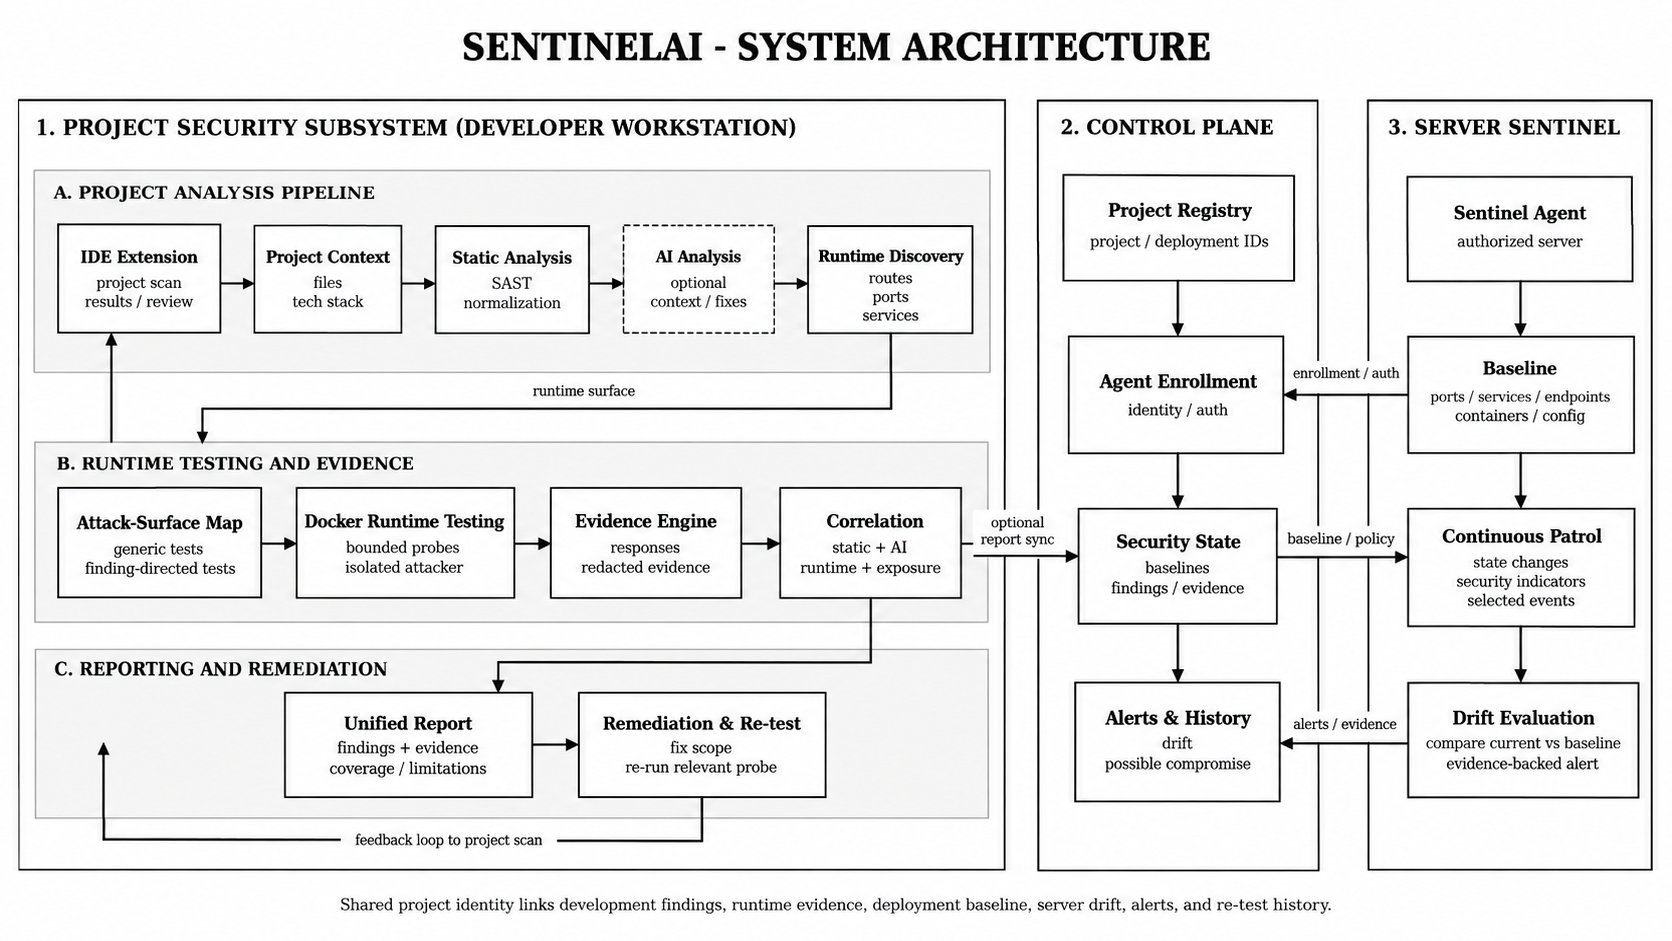
\includegraphics[width=0.95\textwidth]{architecture.png}
\caption{SentinelAI architecture. Project Security and runtime-validation
paths represent the currently implemented workflow, while Server Sentinel
and the Control Plane represent planned components.}
\label{fig:architecture}
\end{figure*}

\subsection{Project Security}

The IDE extension sends normalized project context to the local backend.
Static analyzers produce deterministic findings, while the optional LLM
layer can generate contextual explanations, hypotheses, and remediation
guidance.

Runtime discovery remains independent of source findings. It identifies an
authorized target and attempts to enumerate observable routes, endpoints,
methods, forms, links, and candidate inputs.

The runtime planner creates generic probes and, when relevant source
findings exist, finding-directed probes. Runtime evidence is normalized and
assigned an explicit verdict.

\subsection{Safe Simulation}

Safe Simulation is a controlled runtime-engine regression test. SentinelAI
executes its runtime-security catalogue against a synthetic target with
known expected behavior.

The current catalogue contains 35 runtime-security families. Several
families include multiple controlled variants, resulting in 44 probe
executions in the measured run.

Safe Simulation validates the scanner pipeline and is not treated as a
real-world vulnerability-detection benchmark.

\subsection{Project Runtime Validation}

Project Runtime Validation evaluates an authorized running application.
Unlike Safe Simulation, it determines whether each security family is
applicable before execution.

The workflow is

\begin{equation}
\mathrm{Discovery}
\rightarrow
\mathrm{Applicability}
\rightarrow
\mathrm{Probe}
\rightarrow
\mathrm{Evidence}
\rightarrow
\mathrm{Verdict}.
\label{eq:runtime-flow}
\end{equation}

Generic probes can run even when static and AI findings are empty.
Finding-directed probes can be added when source evidence provides a
specific hypothesis.

For differential tests, SentinelAI preserves

\begin{equation}
\mathrm{Baseline}
\rightarrow
\mathrm{SecurityProbe}
\rightarrow
\mathrm{Comparison}.
\label{eq:baseline-flow}
\end{equation}

Independent probes may execute concurrently through bounded worker
concurrency.

Runtime verdicts are
\textit{confirmed},
\textit{observed exposure},
\textit{inconclusive},
\textit{not reproduced},
\textit{failed}, and
\textit{not applicable}.

Security families requiring unavailable authentication, object ownership,
workflow state, file-upload behavior, GraphQL schemas, WebSocket transport,
concurrency semantics, proxy behavior, callback infrastructure, or cache
state can therefore be classified as not applicable rather than being
executed blindly.

\subsection{Server Sentinel}

Server Sentinel is the planned post-deployment component. It is intended to
observe selected application-facing host state such as listening services,
container state, selected endpoints, and security-relevant configuration.

For project $p$, the approved baseline is

\begin{equation}
B_p=\{b_1,b_2,\ldots,b_n\},
\end{equation}

while the observation at time $t$ is

\begin{equation}
O_p(t)=\{o_1,o_2,\ldots,o_m\}.
\end{equation}

Security drift consists of security-relevant additions, removals, or
attribute changes between $B_p$ and $O_p(t)$.

Server Sentinel and the associated Control Plane remain planned components.

\section{Methodology}

\begin{figure*}[!t]
\centering
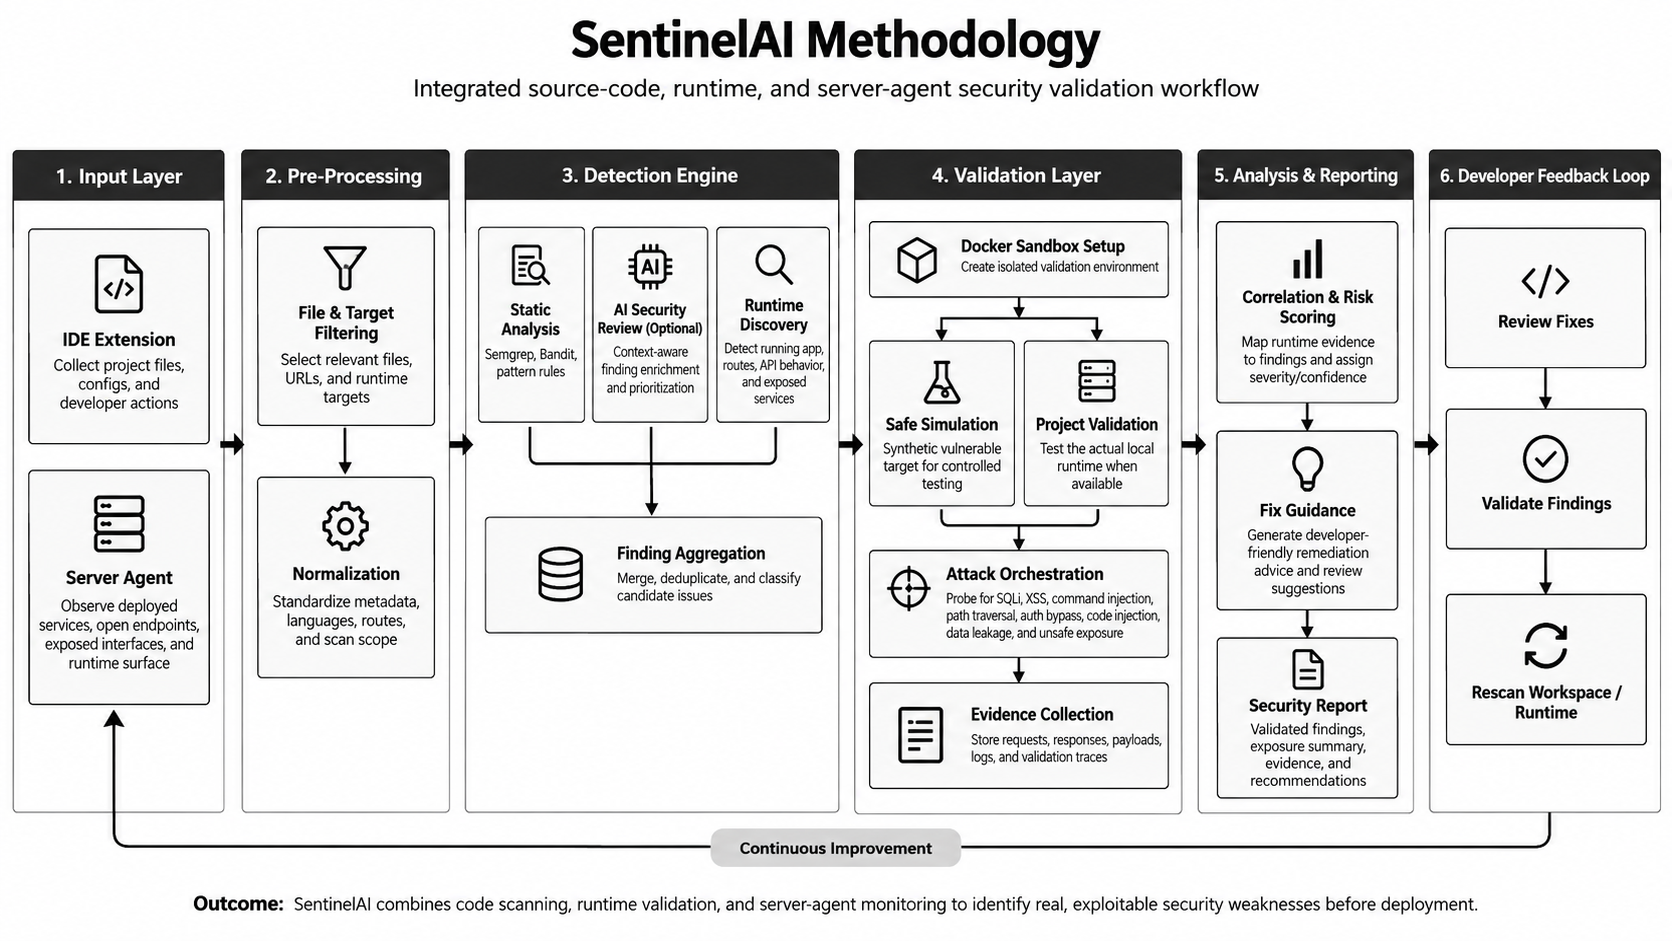
\includegraphics[width=0.95\textwidth]{methodology.png}
\caption{SentinelAI methodology. Project Security, Safe Simulation, and
Project Runtime Validation represent the currently evaluated workflow,
while Server Sentinel monitoring represents planned future work.}
\label{fig:methodology}
\end{figure*}

\subsection{Safe Simulation Method}

Safe Simulation exercises all currently supported runtime-security families
and applicable controlled variants.

The catalogue covers 35 security families spanning injection, file access,
access control, web behavior, HTTP behavior, information exposure, protocol,
and application-context security categories.

The measured Safe Simulation run contains 44 controlled probes across these
35 families.

The synthetic target returns deterministic non-destructive evidence so that
planning, Docker execution, evidence extraction, result normalization,
validation, and verdict generation can be verified.

\subsection{Safe Simulation Reproducibility}

Each Safe Simulation probe is associated with a security family, controlled
target condition, bounded request or observation, expected evidence, and
expected verdict.

A controlled probe is treated as successful when execution completes without
infrastructure failure, evidence is normalized correctly, the observed
verdict matches the predefined expected verdict, and the result maps to the
intended security family.

Multiple variants belonging to the same family are counted separately when
they exercise different request or evidence paths.

For reproducibility, final runs should preserve the SentinelAI source
revision, Node.js and dependency versions, Docker engine version, scanner
and target image identifiers, runtime catalogue version, scenario-to-probe
mapping, expected verdict, observed verdict, and execution status.

\subsection{Project Runtime Validation Method}

Project Runtime Validation begins with authorized runtime discovery and
constructs the available attack surface from observable routes and inputs.

Each security family is evaluated for applicability. A test is executed only
when the target provides sufficient context for a meaningful bounded probe.

This design distinguishes confirmed vulnerability behavior, observable
exposure, inconclusive evidence, absence of the tested signal, execution
failure, and lack of application context.

\subsection{50-Case Report Evaluation}

A set of 50 report-based test cases was used for broader evaluation.
The cases were intentionally heterogeneous: some contained no known
vulnerability, while others contained one or multiple known vulnerabilities.

The distribution is shown in Table~\ref{tab:case-distribution}.

\begin{table}[!t]
\centering
\caption{Distribution of the 50 evaluation test cases.}
\label{tab:case-distribution}
\begin{tabular}{lc}
\toprule
\textbf{Test-Case Type} & \textbf{Number of Cases} \\
\midrule
No known vulnerability & 18 \\
One vulnerability & 15 \\
Two vulnerabilities & 10 \\
Three vulnerabilities & 5 \\
Four vulnerabilities & 2 \\
\midrule
Total & 50 \\
\bottomrule
\end{tabular}
\end{table}

The 32 vulnerable cases contain

\begin{equation}
15+(10\times2)+(5\times3)+(2\times4)=58
\end{equation}

known vulnerability instances.

The remaining 18 cases contain no known vulnerability and are used to
measure whether SentinelAI can correctly avoid raising vulnerability
findings on clean test cases.

The evaluation is performed at two complementary levels. Vulnerability-level
metrics are calculated from the known vulnerability instances and reported
findings. Clean-case classification is evaluated separately using the test
cases that contain no known vulnerabilities. This avoids inflating the
true-negative count by treating every absent vulnerability family as a
separate negative observation.

\subsection{Experimental Outcome Definition}

For Safe Simulation, a probe passes when its observed verdict matches its
predefined expected verdict.

For Project Runtime Validation, results are not interpreted as pass or fail
unless independent vulnerability ground truth is available.

For the 50-case evaluation, a true positive is a known vulnerability
instance correctly reported by SentinelAI. A false negative is a known
vulnerability that SentinelAI failed to report. A false positive is a
reported vulnerability that is not present in the corresponding test case.

At the clean-case level, a true negative is a test case containing no known
vulnerability for which SentinelAI also reports no vulnerability. If one or
more vulnerability findings are produced for a clean case, that case is
counted as a false-positive case.

Duplicate findings mapping to the same case, family, route, and evidence
condition are consolidated before metric calculation.

\subsection{Safety Model}

Runtime probing is restricted to authorized local or project-controlled
targets.

SentinelAI avoids destructive database operations, file deletion,
persistence, brute-force authentication, denial-of-service behavior,
unrestricted remote scanning, and uncontrolled fuzzing.

Docker provides practical execution isolation but shares the host kernel and
is not treated as a complete hardware-security boundary~\cite{b9}.

\section{Implementation}

SentinelAI consists of a Visual Studio Code extension implemented in
TypeScript and a local Node.js/Express backend.

The extension handles workspace interaction, commands, result presentation,
consent, and remediation review. Backend modules handle static analysis,
optional LLM reasoning, runtime discovery, planning, Docker execution,
evidence normalization, validation, correlation, and reporting.

Static analysis can integrate tools such as Bandit, ESLint security rules,
and Semgrep. The LLM layer remains optional.

Safe Simulation executes inside a controlled Docker environment. Project
Runtime Validation allows the controlled attacker environment to reach an
authorized running application while keeping validation execution separate
from the project process.

Runtime evidence can include target URL, request method, response status,
selected headers, response evidence, baseline comparison, security-specific
indicators, and verdict rationale.

\subsection{Implementation Traceability}

\begin{table*}[!t]
\centering
\caption{SentinelAI capability-to-evidence traceability.}
\label{tab:traceability}
\scriptsize
\begin{tabularx}{\textwidth}{p{3.0cm}p{2.2cm}p{4.0cm}X}
\toprule
\textbf{Capability} &
\textbf{Status} &
\textbf{Evidence} &
\textbf{Limitation} \\
\midrule
IDE static analysis &
Implemented &
VS Code extension and backend workflow &
Coverage depends on configured analyzers and supported languages. \\
Optional LLM reasoning &
Implemented &
AI analysis can be enabled or disabled independently &
LLM output is contextual assistance rather than security proof. \\
Independent runtime discovery &
Implemented &
Runtime path operates with zero static or AI findings &
Depth depends on observable routes and project structure. \\
Safe Simulation &
Implemented and measured &
35 families, 44 controlled probes, 44 expected outcomes &
Synthetic engine self-test rather than external benchmark. \\
Project Runtime Validation &
Implemented and measured &
35 families considered and applicability-aware execution &
Application context controls runtime applicability. \\
Evidence verdict model &
Implemented &
Six explicit runtime verdict classes &
Evidence strength varies by family. \\
Bounded parallel execution &
Implemented &
Independent probes execute concurrently &
No formal speed comparison is reported. \\
Remediation and re-test &
Implemented workflow &
Findings can feed remediation and repeated validation &
Developer effectiveness has not yet been formally measured. \\
Context-dependent families &
Partial &
Catalogue and selected validation logic exist &
Some require richer authentication, protocol, proxy, workflow, or state context. \\
Server Sentinel &
Planned &
Baseline and drift architecture defined &
No production-agent performance is claimed. \\
Control Plane &
Planned &
Architecture and data model defined &
Not part of the current evaluated implementation. \\
\bottomrule
\end{tabularx}
\end{table*}

\section{Experimental Design and Metrics}

For labelled classification decisions, let $TP$, $FP$, $TN$, and $FN$
represent true positives, false positives, true negatives, and false
negatives.

\begin{equation}
\mathrm{Precision}
=
\frac{TP}{TP+FP}
\label{eq:precision}
\end{equation}

\begin{equation}
\mathrm{Recall}
=
\frac{TP}{TP+FN}
\label{eq:recall}
\end{equation}

\begin{equation}
\mathrm{Accuracy}
=
\frac{TP+TN}{TP+TN+FP+FN}
\label{eq:accuracy}
\end{equation}

\begin{equation}
F_1
=
2
\frac{\mathrm{Precision}\times\mathrm{Recall}}
{\mathrm{Precision}+\mathrm{Recall}}
\label{eq:f1}
\end{equation}

\begin{equation}
\mathrm{Specificity}
=
\frac{TN}{TN+FP}
\label{eq:specificity}
\end{equation}

\begin{equation}
\mathrm{FPR}
=
\frac{FP}{FP+TN}
\label{eq:fpr}
\end{equation}

\begin{equation}
\mathrm{FNR}
=
\frac{FN}{FN+TP}
\label{eq:fnr}
\end{equation}

The Matthews correlation coefficient is

\begin{equation}
\mathrm{MCC}
=
\frac{TP\cdot TN-FP\cdot FN}
{\sqrt{(TP+FP)(TP+FN)(TN+FP)(TN+FN)}}.
\label{eq:mcc}
\end{equation}

For Safe Simulation,

\begin{equation}
\mathrm{ExpectedOutcomeRate}
=
\frac{P_e}{P},
\label{eq:expected-rate}
\end{equation}

where $P_e$ is the number of probes producing the predefined expected
outcome and $P$ is the total number of controlled probes.

For Project Runtime Validation,

\begin{equation}
\mathrm{RuntimeExecutionCoverage}
=
\frac{F_e}{F},
\label{eq:runtime-coverage}
\end{equation}

where $F_e$ is the number of families issuing HTTP requests and $F$ is the
number of families considered.

\section{Results}

\subsection{Safe Simulation Result}

The expanded Safe Simulation considered all 35 runtime-security families and
executed 44 controlled probes. The run was performed with zero supplied
static or AI findings.

\begin{table}[!t]
\centering
\caption{Measured Safe Simulation result.}
\label{tab:safe-results}
\begin{tabular}{lc}
\toprule
\textbf{Measurement} & \textbf{Observed Value} \\
\midrule
Runtime-security families & 35 \\
Controlled probes & 44 \\
Detected outcomes & 42 \\
Observed exposures & 2 \\
Inconclusive & 0 \\
Failed & 0 \\
Expected outcomes & 44/44 \\
Expected-outcome rate & 100\% \\
Detected-probe rate & 95.45\% \\
Observed-exposure rate & 4.55\% \\
\bottomrule
\end{tabular}
\end{table}

Using Eq.~\eqref{eq:expected-rate},

\begin{equation}
\mathrm{ExpectedOutcomeRate}
=
\frac{44}{44}
=
100\%.
\end{equation}

The detected-probe rate is

\begin{equation}
\frac{42}{44}\times100
=
95.45\%,
\end{equation}

while the observed-exposure rate is

\begin{equation}
\frac{2}{44}\times100
=
4.55\%.
\end{equation}

The two observed-exposure outcomes correspond to controlled debug-exposure
and directory-listing behavior. No controlled probe was inconclusive or
failed.

\subsection{Project Runtime Validation Results}

Project Runtime Validation was evaluated across authorized local project
runtimes using the same applicability-aware runtime catalogue.

For the representative applicability profile reported in the runtime
results, all 35 catalogue families were considered while seven families
generated actual HTTP requests.

\begin{table}[!t]
\centering
\caption{Measured Project Runtime Validation result.}
\label{tab:project-runtime-results}
\begin{tabular}{lc}
\toprule
\textbf{Measurement} & \textbf{Observed Value} \\
\midrule
Security families considered & 35 \\
Families issuing HTTP requests & 7 \\
Confirmed vulnerabilities & 0 \\
Observed exposures & 1 \\
Inconclusive & 1 \\
Not reproduced & 4 \\
Not applicable & 29 \\
Failed & 0 \\
\bottomrule
\end{tabular}
\end{table}

The seven executed families were CORS, security headers, cookie security,
unsafe HTTP methods, sensitive-data exposure, debug exposure, and directory
listing.

The security-header check produced an observed exposure because the response
did not include \texttt{Content-Security-Policy},
\texttt{X-Content-Type-Options}, or
\texttt{Referrer-Policy}.

The unsafe-HTTP-method check was inconclusive because the target responded to
\texttt{OPTIONS} without an \texttt{Allow} header.

CORS, sensitive-data exposure, debug exposure, and directory listing were not
reproduced. Cookie security issued an HTTP request but was ultimately
classified as not applicable because the response did not set a cookie.

The project-specific execution coverage was

\begin{equation}
\mathrm{RuntimeExecutionCoverage}
=
\frac{7}{35}
=
20.00\%.
\end{equation}

This value represents applicability to the tested application rather than
vulnerability-detection accuracy.

\subsection{50-Case Report-Based Evaluation}

The 50-case report evaluation contains 18 clean test cases and 32 vulnerable
test cases. The vulnerable cases contain a total of 58 known vulnerability
instances.

SentinelAI detected 55 of the 58 known vulnerability instances, while three
known vulnerabilities were missed. Five additional vulnerability findings
were classified as false positives.

At the clean-case level, SentinelAI correctly identified 17 of the 18 clean
cases without reporting a vulnerability. One clean test case produced a
false alert. Of the 32 vulnerable cases, at least one correct vulnerability
was identified in 31 cases. Therefore, 48 of the 50 test cases were
classified correctly at the case level.

\begin{table}[!t]
\centering
\caption{Vulnerability-level results across the 50 test cases.}
\label{tab:vulnerability-level-summary}
\begin{tabular}{lc}
\toprule
\textbf{Measurement} & \textbf{Observed Value} \\
\midrule
Total test cases & 50 \\
Clean test cases & 18 \\
Vulnerable test cases & 32 \\
Known vulnerability instances & 58 \\
True positives ($TP$) & 55 \\
False negatives ($FN$) & 3 \\
False-positive findings ($FP$) & 5 \\
\bottomrule
\end{tabular}
\end{table}

Using these vulnerability-level results,

\begin{equation}
\mathrm{Precision}
=
\frac{55}{55+5}
=
91.67\%.
\end{equation}

\begin{equation}
\mathrm{Recall}
=
\frac{55}{55+3}
=
94.83\%.
\end{equation}

\begin{equation}
F_1
=
2
\frac{0.9167\times0.9483}
{0.9167+0.9483}
\approx
93.22\%.
\end{equation}

\begin{table}[!t]
\centering
\caption{Clean-case classification results.}
\label{tab:clean-case-results}
\begin{tabular}{lc}
\toprule
\textbf{Measurement} & \textbf{Observed Value} \\
\midrule
Clean test cases & 18 \\
Correctly identified clean cases ($TN$) & 17 \\
Clean cases with false alerts & 1 \\
\bottomrule
\end{tabular}
\end{table}

The clean-case specificity is

\begin{equation}
\mathrm{Specificity}_{case}
=
\frac{17}{18}
=
94.44\%.
\end{equation}

The clean-case false-positive rate is

\begin{equation}
\mathrm{FPR}_{case}
=
\frac{1}{18}
=
5.56\%.
\end{equation}

The case-level accuracy is

\begin{equation}
\mathrm{CaseAccuracy}
=
\frac{48}{50}
=
96.00\%.
\end{equation}

\begin{table}[!t]
\centering
\caption{Summary of the 50-case SentinelAI evaluation.}
\label{tab:50-case-metrics}
\begin{tabular}{lc}
\toprule
\textbf{Metric} & \textbf{Value} \\
\midrule
Test cases & 50 \\
Known vulnerability instances & 58 \\
True positives & 55 \\
False negatives & 3 \\
False-positive findings & 5 \\
Clean-case true negatives & 17 \\
Precision & 91.67\% \\
Recall & 94.83\% \\
F1-score & 93.22\% \\
Clean-case specificity & 94.44\% \\
Clean-case false-positive rate & 5.56\% \\
Case-level accuracy & 96.00\% \\
\bottomrule
\end{tabular}
\end{table}

\subsection{Vulnerability-Level Results}

\begin{table*}[!t]
\centering
\caption{Vulnerability-level results from the 50-case evaluation.}
\label{tab:vulnerability-results}
\scriptsize
\begin{tabularx}{\textwidth}{Xcccc}
\toprule
\textbf{Vulnerability Family} &
\textbf{Ground Truth} &
\textbf{Detected} &
\textbf{Missed} &
\textbf{False Alerts} \\
\midrule
SQL Injection & 2 & 2 & 0 & 0 \\
NoSQL Injection & 2 & 2 & 0 & 0 \\
Cross-Site Scripting & 2 & 2 & 0 & 1 \\
Command Injection & 2 & 2 & 0 & 0 \\
Code Injection & 1 & 1 & 0 & 0 \\
SSTI & 2 & 2 & 0 & 0 \\
Path Traversal & 2 & 2 & 0 & 0 \\
Local File Inclusion & 2 & 2 & 0 & 0 \\
SSRF & 2 & 1 & 1 & 0 \\
Open Redirect & 2 & 2 & 0 & 0 \\
Authentication Bypass & 2 & 2 & 0 & 0 \\
IDOR/BOLA & 2 & 2 & 0 & 0 \\
JWT Security & 1 & 1 & 0 & 0 \\
CORS & 2 & 2 & 0 & 1 \\
Security Headers & 2 & 2 & 0 & 1 \\
Cookie Security & 1 & 1 & 0 & 0 \\
Sensitive Data Exposure & 2 & 2 & 0 & 0 \\
Debug Exposure & 2 & 2 & 0 & 0 \\
Unsafe HTTP Methods & 2 & 2 & 0 & 1 \\
Directory Listing & 1 & 1 & 0 & 0 \\
LDAP Injection & 1 & 1 & 0 & 0 \\
XPath Injection & 1 & 1 & 0 & 0 \\
XXE & 1 & 1 & 0 & 0 \\
Prototype Pollution & 1 & 1 & 0 & 0 \\
Insecure Deserialization & 1 & 1 & 0 & 0 \\
Unsafe File Upload & 2 & 2 & 0 & 0 \\
CSRF & 1 & 1 & 0 & 0 \\
Mass Assignment & 2 & 2 & 0 & 0 \\
Race Condition & 2 & 1 & 1 & 0 \\
Business Logic Flaw & 2 & 2 & 0 & 0 \\
Host Header Injection & 1 & 1 & 0 & 0 \\
WebSocket Security & 1 & 1 & 0 & 0 \\
GraphQL Security & 2 & 1 & 1 & 0 \\
HTTP Request Smuggling & 2 & 2 & 0 & 1 \\
Cache Poisoning & 2 & 2 & 0 & 0 \\
\midrule
\textbf{Total} & \textbf{58} & \textbf{55} & \textbf{3} & \textbf{5} \\
\bottomrule
\end{tabularx}
\end{table*}

The three missed vulnerability instances occur in SSRF, race-condition, and
GraphQL scenarios, which require additional application, state, or protocol
context for reliable validation.

False-positive findings are concentrated in a small number of web and
HTTP-oriented categories, while the overall vulnerability-level precision
and recall remain above 90\%.

\section{Limitations}

Safe Simulation validates controlled engine behavior and should not be
generalized directly to arbitrary production applications.

The synthetic target intentionally provides known evidence, so the 44-of-44
result demonstrates integration and regression correctness rather than
universal vulnerability-detection capability.

Project Runtime Validation remains application-dependent. Projects with
limited server-side behavior naturally provide less context for categories
requiring authentication, database inputs, GraphQL, WebSockets, file
uploads, workflows, reverse-proxy behavior, concurrency, or cache state.

The 50-case evaluation separates vulnerability-level detection from
clean-case classification. Precision, recall, and F1-score are calculated
from known vulnerability instances, while specificity and clean-case false
positive rate are calculated from intentionally clean test cases. This
avoids artificially inflating the true-negative count.

The optional LLM layer inherits known limitations including hallucination,
context errors, inconsistent reasoning, and prompt injection
~\cite{b4,b13}.

Several runtime families still require richer application context before
they can be considered broadly operational on arbitrary projects.

Server Sentinel remains planned, and no production-agent performance is
claimed.

Docker improves execution isolation but shares the host kernel and should
not be treated as a complete security boundary~\cite{b9}.

\section{Discussion}

The strongest current contribution of SentinelAI is the separation of
scanner self-testing from real-project runtime validation.

Safe Simulation verifies that the runtime engine can plan, execute,
normalize, and classify controlled scenarios even when static and AI
findings are absent.

Project Runtime Validation demonstrates that catalogue size should not be
confused with the number of tests that should execute against a particular
application. Applicability filtering prevents irrelevant probes from being
interpreted as failed detections.

The 50-case evaluation extends the analysis across a broader set of report-based
project scenarios and includes both vulnerable and clean test cases. The result shows
high recall while maintaining a low false-positive rate, while the three
missed instances identify areas where additional contextual or
protocol-specific support remains useful.

The explicit verdict model improves interpretability by distinguishing
confirmed behavior from exposure, uncertainty, absence of a signal,
execution failure, and lack of applicability.

\section{Ethical and Security Considerations}

SentinelAI is intended only for applications and infrastructure that the
user owns or is explicitly authorized to test.

Runtime probes are bounded and non-destructive. SentinelAI should not
automatically perform destructive exploitation, persistence, brute-force
credential attacks, denial-of-service testing, unrestricted remote scanning,
or uncontrolled fuzzing.

Sensitive values including credentials, tokens, environment variables, and
personal data should be redacted from retained evidence and generated
reports where appropriate.

\section{Conclusion}

SentinelAI integrates IDE-based source analysis, optional AI reasoning,
independent runtime discovery, applicability-aware runtime validation,
evidence-based verdicts, remediation and re-test, and a planned
post-deployment monitoring architecture.

The measured Safe Simulation experiment considered 35 runtime-security
families and executed 44 controlled probes. All 44 produced their expected
outcomes, including 42 detected outcomes and two observed exposures, with no
inconclusive or failed executions.

Project Runtime Validation separately applies the 35-family catalogue to
authorized project runtimes using applicability-aware execution. In the
reported applicability profile, seven families generated HTTP requests,
producing one observed exposure, one inconclusive result, four
not-reproduced results, 29 not-applicable verdicts, and zero failures.

The broader 50-case report-based evaluation contained 18 clean test cases
and 32 vulnerable test cases, representing 58 known vulnerability instances.
SentinelAI detected 55 of the 58 known vulnerabilities, with three misses
and five false-positive findings. This corresponds to 91.67\% precision,
94.83\% recall, and 93.22\% F1-score. At the case level, 17 of 18 clean
cases were correctly identified as clean, giving 94.44\% clean-case
specificity, while 48 of the 50 total test cases were classified correctly,
giving 96.00\% case-level accuracy.

These results indicate promising performance while also showing that
context-dependent categories such as SSRF, race conditions, and GraphQL
security remain areas for further development.

The next stage of work is reproducible repeated evaluation across additional
applications and labelled security benchmarks, followed by implementation
and controlled evaluation of Server Sentinel.

\section{Future Work}

Future work includes authenticated crawling, session and token context,
improved API discovery, deeper source analysis, broader language support,
and stronger real-project runtime execution for context-dependent security
families.

Priority areas include authenticated IDOR/BOLA testing, JWT/session context,
controlled SSRF callbacks, GraphQL discovery, WebSocket transport, safe
file-upload lifecycle testing, concurrency testing for race conditions,
workflow-aware business-logic testing, proxy-aware request-smuggling
analysis, and cache-aware validation.

Runtime evaluation should additionally include OWASP Benchmark, NIST
SARD/Juliet, OWASP Juice Shop, and WebGoat where technically applicable,
together with a controlled OWASP ZAP comparison.

Server Sentinel future work includes authenticated enrollment, approved
deployment baselines, secure agent communication, service and container
observation, controlled drift injection, repeated measurements, and
multi-project monitoring.

\section*{Acknowledgment}

The authors thank Prof. Vidya Sagvekar, Department of AI \& Data Science,
K.J. Somaiya Institute of Technology, for project guidance and academic
supervision.

\begin{thebibliography}{00}

\bibitem{b4}
Y.~Liu, G.~Deng, Z.~Li, Y.~Wang, Z.~Zhang, W.~Liu, T.~Wang,
Y.~Zheng, and Y.~Liu,
``Prompt Injection Attacks Against Large Language Models,''
\textit{arXiv preprint arXiv:2306.05499}, 2023.

\bibitem{b5}
X.~Yuan, L.~Peng, Y.~Luo, and J.~Liu,
``A Static Detection Method for SQL Injection Vulnerability Based on Program Transformation,''
\textit{Applied Sciences}, 2023.

\bibitem{b7}
G.~Deng, Y.~Liu, V.~Mayoral-Vilches, P.~Liu, Y.~Li, Y.~Xu,
T.~Zhang, Y.~Liu, M.~Pinzger, and S.~Rass,
``PentestGPT: Evaluating and Harnessing Large Language Models for Automated Penetration Testing,''
in \textit{33rd USENIX Security Symposium (USENIX Security 24)},
pp.~847--864, 2024.

\bibitem{b8}
A.~Happe and J.~Cito,
``Getting pwn'd by AI: Penetration Testing with Large Language Models,''
in \textit{Proc. ACM Joint European Software Engineering Conference and Symposium on the Foundations of Software Engineering (ESEC/FSE)},
2023.

\bibitem{b9}
W.~Jiang and Z.~Li,
``Vulnerability Analysis and Security Research of Docker Container,''
in \textit{Proc. 2020 IEEE 3rd International Conference on Information Systems and Computer Aided Education (ICISCAE)},
pp.~354--357, 2020.

\bibitem{b10}
E.~Pelofske, G.~Hahn, and H.~Djidjev,
``Automated Software Vulnerability Static Code Analysis Using Generative Pre-Trained Transformer Models,''
\textit{arXiv preprint arXiv:2408.00197}, 2024.

\bibitem{b11}
Z.~Li, S.~Dutta, and M.~Naik,
``LLM-Assisted Static Analysis for Detecting Security Vulnerabilities,''
\textit{arXiv preprint arXiv:2405.17238}, 2024.

\bibitem{b13}
S.~Ullah, M.~Han, S.~Pujar, H.~Pearce, A.~Coskun,
and G.~Stringhini,
``LLMs Cannot Reliably Identify and Reason About Security Vulnerabilities (Yet?): A Comprehensive Evaluation, Framework, and Benchmarks,''
in \textit{2024 IEEE Symposium on Security and Privacy},
pp.~862--880, 2024.

\bibitem{b14}
N.~Shiri Harzevili, A.~Boaye Belle, J.~Wang, S.~Wang,
Z.~M.~J.~Jiang, and N.~Nagappan,
``A Systematic Literature Review on Automated Software Vulnerability Detection Using Machine Learning,''
\textit{ACM Computing Surveys}, vol.~57, no.~3, 2024.

\bibitem{datadogagent}
Datadog,
``Agent Data Security,''
\textit{Datadog Documentation}.
[Online]. Available:
\url{https://docs.datadoghq.com/data_security/agent/}.
Accessed: Oct.~8, 2026.

\bibitem{wazuhagent}
Wazuh,
``Wazuh Agent,''
\textit{Wazuh Documentation}.
[Online]. Available:
\url{https://documentation.wazuh.com/current/user-manual/agent/index.html}.
Accessed: Oct.~8, 2026.

\bibitem{zap}
OWASP ZAP Development Team,
``Automation Framework,''
\textit{OWASP ZAP Documentation}.
[Online]. Available:
\url{https://www.zaproxy.org/docs/automate/automation-framework/}.
Accessed: Oct.~8, 2026.

\bibitem{nuclei}
ProjectDiscovery,
``Nuclei Documentation.''
[Online]. Available:
\url{https://docs.projectdiscovery.io/opensource/nuclei/overview}.
Accessed: Oct.~8, 2026.

\bibitem{falco}
The Falco Project,
``Falco Documentation.''
[Online]. Available:
\url{https://falco.org/docs/}.
Accessed: Oct.~8, 2026.

\bibitem{osquery}
The osquery Project,
``osquery: Performant Endpoint Visibility.''
[Online]. Available:
\url{https://osquery.io/}.
Accessed: Oct.~8, 2026.

\end{thebibliography}

\end{document}